\documentclass[twoside]{book}

% Packages required by doxygen
\usepackage{calc}
\usepackage{doxygen}
\usepackage{graphicx}
\usepackage[utf8]{inputenc}
\usepackage{makeidx}
\usepackage{multicol}
\usepackage{multirow}
\usepackage{textcomp}
\usepackage[table]{xcolor}

% Font selection
\usepackage[T1]{fontenc}
\usepackage{mathptmx}
\usepackage[scaled=.90]{helvet}
\usepackage{courier}
\usepackage{amssymb}
\usepackage{sectsty}
\renewcommand{\familydefault}{\sfdefault}
\allsectionsfont{%
  \fontseries{bc}\selectfont%
  \color{darkgray}%
}
\renewcommand{\DoxyLabelFont}{%
  \fontseries{bc}\selectfont%
  \color{darkgray}%
}

% Page & text layout
\usepackage{geometry}
\geometry{%
  a4paper,%
  top=2.5cm,%
  bottom=2.5cm,%
  left=2.5cm,%
  right=2.5cm%
}
\tolerance=750
\hfuzz=15pt
\hbadness=750
\setlength{\emergencystretch}{15pt}
\setlength{\parindent}{0cm}
\setlength{\parskip}{0.2cm}
\makeatletter
\renewcommand{\paragraph}{%
  \@startsection{paragraph}{4}{0ex}{-1.0ex}{1.0ex}{%
    \normalfont\normalsize\bfseries\SS@parafont%
  }%
}
\renewcommand{\subparagraph}{%
  \@startsection{subparagraph}{5}{0ex}{-1.0ex}{1.0ex}{%
    \normalfont\normalsize\bfseries\SS@subparafont%
  }%
}
\makeatother

% Headers & footers
\usepackage{fancyhdr}
\pagestyle{fancyplain}
\fancyhead[LE]{\fancyplain{}{\bfseries\thepage}}
\fancyhead[CE]{\fancyplain{}{}}
\fancyhead[RE]{\fancyplain{}{\bfseries\leftmark}}
\fancyhead[LO]{\fancyplain{}{\bfseries\rightmark}}
\fancyhead[CO]{\fancyplain{}{}}
\fancyhead[RO]{\fancyplain{}{\bfseries\thepage}}
\fancyfoot[LE]{\fancyplain{}{}}
\fancyfoot[CE]{\fancyplain{}{}}
\fancyfoot[RE]{\fancyplain{}{\bfseries\scriptsize Generated on Mon Oct 6 2014 14\-:38\-:49 for My Project by Doxygen }}
\fancyfoot[LO]{\fancyplain{}{\bfseries\scriptsize Generated on Mon Oct 6 2014 14\-:38\-:49 for My Project by Doxygen }}
\fancyfoot[CO]{\fancyplain{}{}}
\fancyfoot[RO]{\fancyplain{}{}}
\renewcommand{\footrulewidth}{0.4pt}
\renewcommand{\chaptermark}[1]{%
  \markboth{#1}{}%
}
\renewcommand{\sectionmark}[1]{%
  \markright{\thesection\ #1}%
}

% Indices & bibliography
\usepackage{natbib}
\usepackage[titles]{tocloft}
\setcounter{tocdepth}{3}
\setcounter{secnumdepth}{5}
\makeindex

% Hyperlinks (required, but should be loaded last)
\usepackage{ifpdf}
\ifpdf
  \usepackage[pdftex,pagebackref=true]{hyperref}
\else
  \usepackage[ps2pdf,pagebackref=true]{hyperref}
\fi
\hypersetup{%
  colorlinks=true,%
  linkcolor=blue,%
  citecolor=blue,%
  unicode%
}

% Custom commands
\newcommand{\clearemptydoublepage}{%
  \newpage{\pagestyle{empty}\cleardoublepage}%
}


%===== C O N T E N T S =====

\begin{document}

% Titlepage & ToC
\hypersetup{pageanchor=false}
\pagenumbering{roman}
\begin{titlepage}
\vspace*{7cm}
\begin{center}%
{\Large My Project }\\
\vspace*{1cm}
{\large Generated by Doxygen 1.8.6}\\
\vspace*{0.5cm}
{\small Mon Oct 6 2014 14:38:49}\\
\end{center}
\end{titlepage}
\clearemptydoublepage
\tableofcontents
\clearemptydoublepage
\pagenumbering{arabic}
\hypersetup{pageanchor=true}

%--- Begin generated contents ---
\chapter{Projeto Canvas}
\label{index}\hypertarget{index}{}\hypertarget{index_intro_sec}{}\section{Introdução}\label{index_intro_sec}
Documentação dos códigos usados para desenvolver o sistema de login e cadastro do Canvas. 
\chapter{Hierarchical Index}
\section{Class Hierarchy}
This inheritance list is sorted roughly, but not completely, alphabetically\-:\begin{DoxyCompactList}
\item C\-I\-\_\-\-Controller\begin{DoxyCompactList}
\item \contentsline{section}{Login}{\pageref{classLogin}}{}
\item \contentsline{section}{Members}{\pageref{classMembers}}{}
\item \contentsline{section}{Welcome}{\pageref{classWelcome}}{}
\end{DoxyCompactList}
\item C\-I\-\_\-\-Model\begin{DoxyCompactList}
\item \contentsline{section}{Login\-\_\-model}{\pageref{classLogin__model}}{}
\item \contentsline{section}{Members\-\_\-model}{\pageref{classMembers__model}}{}
\end{DoxyCompactList}
\end{DoxyCompactList}

\chapter{Class Index}
\section{Class List}
Here are the classes, structs, unions and interfaces with brief descriptions\-:\begin{DoxyCompactList}
\item\contentsline{section}{\hyperlink{classLogin}{Login} \\*Soliciata a realização do login e logout }{\pageref{classLogin}}{}
\item\contentsline{section}{\hyperlink{classLogin__model}{Login\-\_\-model} \\*Realização do login e logout }{\pageref{classLogin__model}}{}
\item\contentsline{section}{\hyperlink{classMembers}{Members} \\*Mostra, cadastra, edita, apaga e valida os usuarios }{\pageref{classMembers}}{}
\item\contentsline{section}{\hyperlink{classMembers__model}{Members\-\_\-model} \\*Busca, cadastra, edita, apaga e valida os usuarios no banco }{\pageref{classMembers__model}}{}
\item\contentsline{section}{\hyperlink{classWelcome}{Welcome} \\*Nativa do Codeigniter }{\pageref{classWelcome}}{}
\end{DoxyCompactList}

\chapter{File Index}
\section{File List}
Here is a list of all documented files with brief descriptions\-:\begin{DoxyCompactList}
\item\contentsline{section}{application/controllers/\hyperlink{login_8php}{login.\-php} \\*Sistema de login do canvas }{\pageref{login_8php}}{}
\item\contentsline{section}{application/controllers/\hyperlink{members_8php}{members.\-php} \\*Sistema de login do canvas }{\pageref{members_8php}}{}
\item\contentsline{section}{application/models/\hyperlink{login__model_8php}{login\-\_\-model.\-php} \\*Sistema de login do canvas }{\pageref{login__model_8php}}{}
\item\contentsline{section}{application/models/\hyperlink{members__model_8php}{members\-\_\-model.\-php} \\*Sistema de login do canvas }{\pageref{members__model_8php}}{}
\end{DoxyCompactList}

\chapter{Class Documentation}
\hypertarget{classLogin}{\section{Login Class Reference}
\label{classLogin}\index{Login@{Login}}
}


Soliciata a realização do login e logout.  


Inheritance diagram for Login\-:\begin{figure}[H]
\begin{center}
\leavevmode
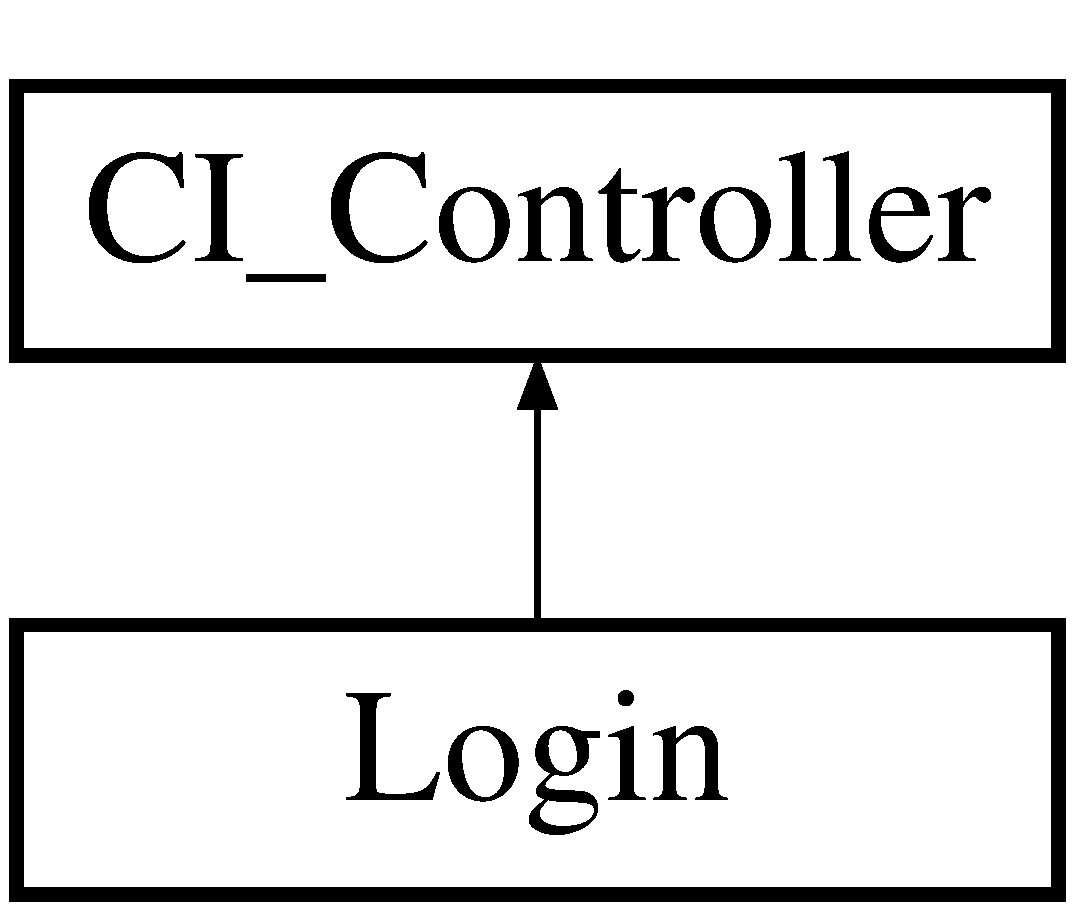
\includegraphics[height=2.000000cm]{classLogin}
\end{center}
\end{figure}
\subsection*{Public Member Functions}
\begin{DoxyCompactItemize}
\item 
\hypertarget{classLogin_a1c32d6f7816f8912e52bb554035fbf14}{\hyperlink{classLogin_a1c32d6f7816f8912e52bb554035fbf14}{\-\_\-\-\_\-construct} ()}\label{classLogin_a1c32d6f7816f8912e52bb554035fbf14}

\begin{DoxyCompactList}\small\item\em Chama a biblioteca U\-R\-L do codeigniter. \end{DoxyCompactList}\item 
\hyperlink{classLogin_a2eed7119960cf8499981ed4c3678345e}{index} ()
\begin{DoxyCompactList}\small\item\em Analisa se existe sessão aberta. \end{DoxyCompactList}\item 
\hyperlink{classLogin_a8a46e12700d878082ecb6a42bda5be9b}{try\-Login} ()
\begin{DoxyCompactList}\small\item\em Realiza o login. \end{DoxyCompactList}\item 
\hyperlink{classLogin_ae939c3bb65c459e67058c4dd5910aa56}{log\-Out} ()
\begin{DoxyCompactList}\small\item\em Realiza o logout da sessão. \end{DoxyCompactList}\end{DoxyCompactItemize}


\subsection{Detailed Description}
Soliciata a realização do login e logout. 

\subsection{Member Function Documentation}
\hypertarget{classLogin_a2eed7119960cf8499981ed4c3678345e}{\index{Login@{Login}!index@{index}}
\index{index@{index}!Login@{Login}}
\subsubsection[{index}]{\setlength{\rightskip}{0pt plus 5cm}Login\-::index (
\begin{DoxyParamCaption}
{}
\end{DoxyParamCaption}
)}}\label{classLogin_a2eed7119960cf8499981ed4c3678345e}


Analisa se existe sessão aberta. 

Chama a biblioteca Session do Codeigniter.

Caso não exista sessão aberta é redirecionado para a página de login. 
\begin{DoxyParams}{Parameters}
{\em logged} & \\
\hline
\end{DoxyParams}
caso a sessão esteja iniciada redireciona para a página principal.

Carrega a login\-\_\-model.

Recebe o email da login\-\_\-model.

Analisa o privilegio do usuario. \hypertarget{classLogin_ae939c3bb65c459e67058c4dd5910aa56}{\index{Login@{Login}!log\-Out@{log\-Out}}
\index{log\-Out@{log\-Out}!Login@{Login}}
\subsubsection[{log\-Out}]{\setlength{\rightskip}{0pt plus 5cm}Login\-::log\-Out (
\begin{DoxyParamCaption}
{}
\end{DoxyParamCaption}
)}}\label{classLogin_ae939c3bb65c459e67058c4dd5910aa56}


Realiza o logout da sessão. 

Chama a biblioteca Session.

Destroy a sessão.

Redireciona para a página de login. \hypertarget{classLogin_a8a46e12700d878082ecb6a42bda5be9b}{\index{Login@{Login}!try\-Login@{try\-Login}}
\index{try\-Login@{try\-Login}!Login@{Login}}
\subsubsection[{try\-Login}]{\setlength{\rightskip}{0pt plus 5cm}Login\-::try\-Login (
\begin{DoxyParamCaption}
{}
\end{DoxyParamCaption}
)}}\label{classLogin_a8a46e12700d878082ecb6a42bda5be9b}


Realiza o login. 

Checa se o email e senha informado estão conforme os padrões para os mesmo.

Caso estejam redirecionam para a login\-\_\-model, passaso o email e senha informados.

Se o banco retornar True, para a vefiricação do login no banco, o usuario é redirecionado para a página inicial.

Caso retorne false, o usuario é redirecionado para a página de login. 

The documentation for this class was generated from the following file\-:\begin{DoxyCompactItemize}
\item 
application/controllers/\hyperlink{login_8php}{login.\-php}\end{DoxyCompactItemize}

\hypertarget{classLogin__model}{\section{Login\-\_\-model Class Reference}
\label{classLogin__model}\index{Login\-\_\-model@{Login\-\_\-model}}
}


realização do login e logout.  


Inheritance diagram for Login\-\_\-model\-:\begin{figure}[H]
\begin{center}
\leavevmode
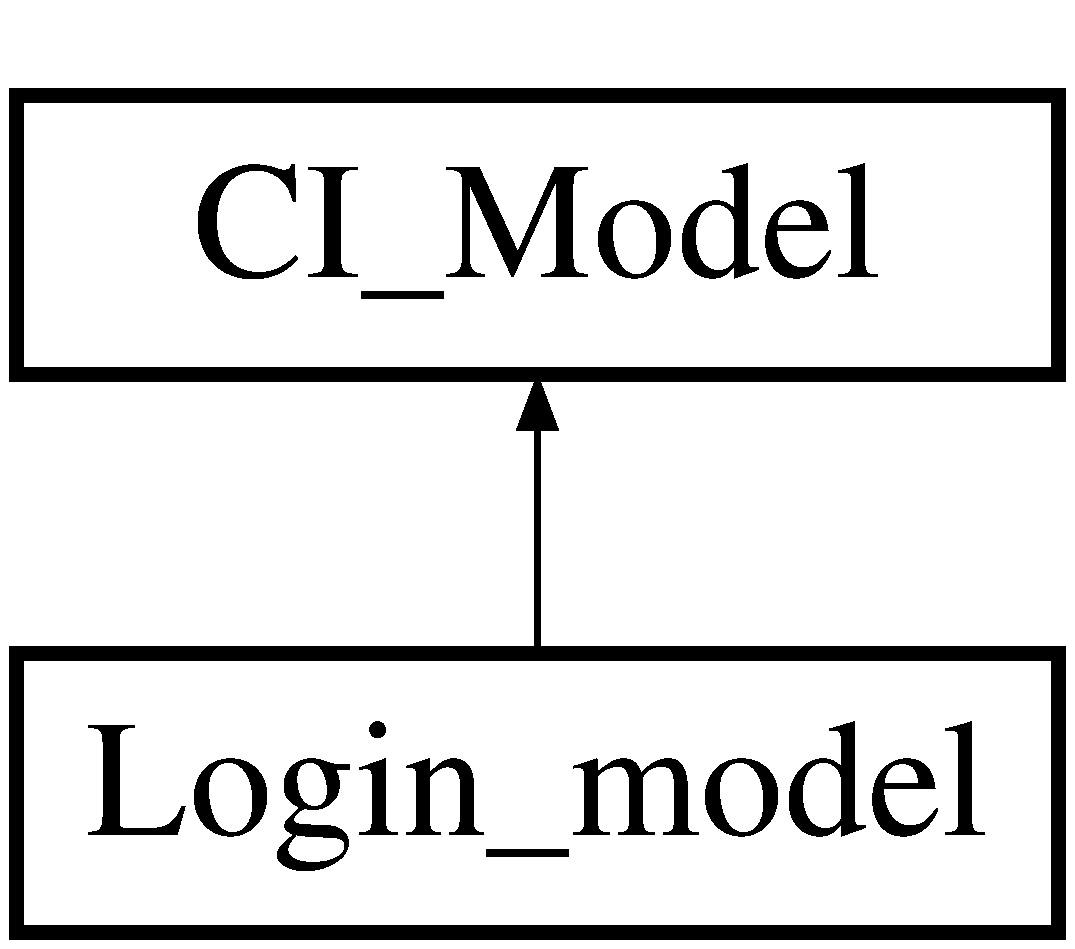
\includegraphics[height=2.000000cm]{classLogin__model}
\end{center}
\end{figure}
\subsection*{Public Member Functions}
\begin{DoxyCompactItemize}
\item 
\hyperlink{classLogin__model_ad77c9bf41acd559ece8594aba412f515}{validate\-User} (\$email, \$password)
\begin{DoxyCompactList}\small\item\em Valida o usuario. \end{DoxyCompactList}\item 
\hyperlink{classLogin__model_a2caeb6464acaa460860fd51b8a0ea6b2}{get\-User\-Data} (\$email)
\end{DoxyCompactItemize}


\subsection{Detailed Description}
realização do login e logout. 

\subsection{Member Function Documentation}
\hypertarget{classLogin__model_a2caeb6464acaa460860fd51b8a0ea6b2}{\index{Login\-\_\-model@{Login\-\_\-model}!get\-User\-Data@{get\-User\-Data}}
\index{get\-User\-Data@{get\-User\-Data}!Login_model@{Login\-\_\-model}}
\subsubsection[{get\-User\-Data}]{\setlength{\rightskip}{0pt plus 5cm}Login\-\_\-model\-::get\-User\-Data (
\begin{DoxyParamCaption}
\item[{}]{\$email}
\end{DoxyParamCaption}
)}}\label{classLogin__model_a2caeb6464acaa460860fd51b8a0ea6b2}
Busca os dados do usuario. 
\begin{DoxyParams}{Parameters}
{\em email} & \\
\hline
\end{DoxyParams}
Os dados obtidos no banco criam o objeto Member

\begin{DoxyReturn}{Returns}
member 
\end{DoxyReturn}
\hypertarget{classLogin__model_ad77c9bf41acd559ece8594aba412f515}{\index{Login\-\_\-model@{Login\-\_\-model}!validate\-User@{validate\-User}}
\index{validate\-User@{validate\-User}!Login_model@{Login\-\_\-model}}
\subsubsection[{validate\-User}]{\setlength{\rightskip}{0pt plus 5cm}Login\-\_\-model\-::validate\-User (
\begin{DoxyParamCaption}
\item[{}]{\$email, }
\item[{}]{\$password}
\end{DoxyParamCaption}
)}}\label{classLogin__model_ad77c9bf41acd559ece8594aba412f515}


Valida o usuario. 

Procura o email.

Procura a senha.

Pega dados da tabela Cadastros onde há esse login e senha.

Confirma se há 1 registro para esses dados no banco.

Caso verdadeiro\-: \begin{DoxyReturn}{Returns}
true 
\end{DoxyReturn}


The documentation for this class was generated from the following file\-:\begin{DoxyCompactItemize}
\item 
application/models/\hyperlink{login__model_8php}{login\-\_\-model.\-php}\end{DoxyCompactItemize}

\hypertarget{classMembers}{\section{Members Class Reference}
\label{classMembers}\index{Members@{Members}}
}


Mostra, cadastra, edita, apaga e valida os usuarios.  


Inheritance diagram for Members\-:\begin{figure}[H]
\begin{center}
\leavevmode
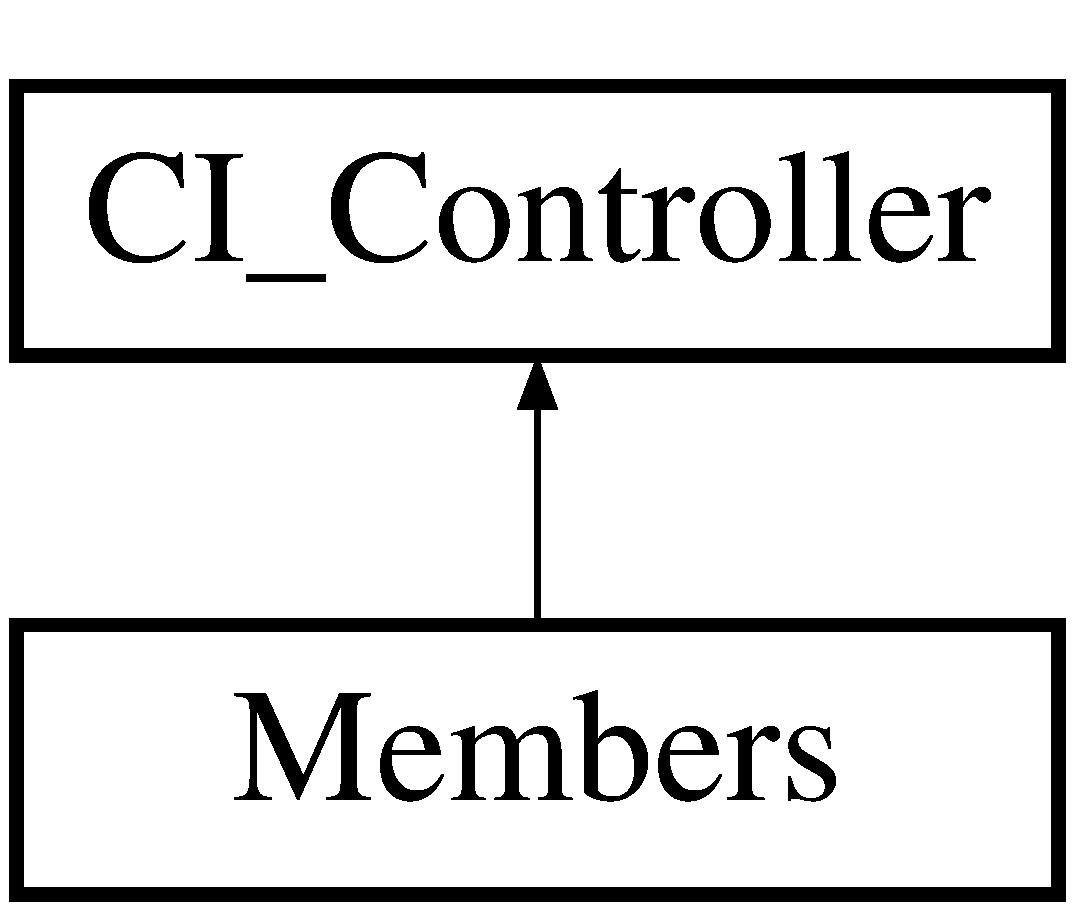
\includegraphics[height=2.000000cm]{classMembers}
\end{center}
\end{figure}
\subsection*{Public Member Functions}
\begin{DoxyCompactItemize}
\item 
\hypertarget{classMembers_a6b8071cbd5837e99c283880ea9fdb695}{\hyperlink{classMembers_a6b8071cbd5837e99c283880ea9fdb695}{\-\_\-\-\_\-construct} ()}\label{classMembers_a6b8071cbd5837e99c283880ea9fdb695}

\begin{DoxyCompactList}\small\item\em Chama a bibilioteca U\-R\-L do codeigniter. \end{DoxyCompactList}\item 
\hyperlink{classMembers_a97543c7a9581814294ca85ccba384b64}{get\-All} (\$msg=N\-U\-L\-L)
\item 
\hyperlink{classMembers_ac2012deacee8545968300b8790b17664}{add\-Member} ()
\begin{DoxyCompactList}\small\item\em Redireciona para a view de cadastro de novos membros. \end{DoxyCompactList}\item 
\hyperlink{classMembers_a82f4446426e827d31bb951375ce64511}{validate\-Member} ()
\begin{DoxyCompactList}\small\item\em Analisa se os dados informados no cadastro de novos membros são validos. \end{DoxyCompactList}\item 
\hyperlink{classMembers_a587c1356d4e780d41a96cdbbee9c7fa9}{edit} (\$login)
\item 
\hyperlink{classMembers_a51f276a9b719cfb75b76c74806d2ece1}{validate\-Update} (\$login)
\item 
\hyperlink{classMembers_a2d5709b313f19375a6642d93b99c3661}{delete} (\$login)
\end{DoxyCompactItemize}


\subsection{Detailed Description}
Mostra, cadastra, edita, apaga e valida os usuarios. 

\subsection{Member Function Documentation}
\hypertarget{classMembers_ac2012deacee8545968300b8790b17664}{\index{Members@{Members}!add\-Member@{add\-Member}}
\index{add\-Member@{add\-Member}!Members@{Members}}
\subsubsection[{add\-Member}]{\setlength{\rightskip}{0pt plus 5cm}Members\-::add\-Member (
\begin{DoxyParamCaption}
{}
\end{DoxyParamCaption}
)}}\label{classMembers_ac2012deacee8545968300b8790b17664}


Redireciona para a view de cadastro de novos membros. 

Verifica se a sessão está aberta.

Caso esteja, carrega a login\-\_\-model.

Verifica o privilegio do usuário.

Caso Admin, redireciona para a view registration\-\_\-form\-\_\-view, para realizar o novo cadastro.

Caso manager, redireciona para a view registration\-\_\-form\-\_\-view, para realizar o novo cadastro.

Caso Worker, não permite adicionar novas membros. \hypertarget{classMembers_a2d5709b313f19375a6642d93b99c3661}{\index{Members@{Members}!delete@{delete}}
\index{delete@{delete}!Members@{Members}}
\subsubsection[{delete}]{\setlength{\rightskip}{0pt plus 5cm}Members\-::delete (
\begin{DoxyParamCaption}
\item[{}]{\$login}
\end{DoxyParamCaption}
)}}\label{classMembers_a2d5709b313f19375a6642d93b99c3661}
Responsavel por deletar cadastros. 
\begin{DoxyParams}{Parameters}
{\em login} & \\
\hline
\end{DoxyParams}
Verifica se a sessão está aberta.

Caso esteja, carrega a login\-\_\-model.

Checa o privilegio do usuário. Verificasse usuário possue privilegio igual ou superior ou que deseja deletar. Caso não possua, é mostrado uma mensagem de alerta. caso possua, a members\-\_\-model é carregada, se o cadastro for deletado corretamente é mostrado uma mensagem de sucesso. \hypertarget{classMembers_a587c1356d4e780d41a96cdbbee9c7fa9}{\index{Members@{Members}!edit@{edit}}
\index{edit@{edit}!Members@{Members}}
\subsubsection[{edit}]{\setlength{\rightskip}{0pt plus 5cm}Members\-::edit (
\begin{DoxyParamCaption}
\item[{}]{\$login}
\end{DoxyParamCaption}
)}}\label{classMembers_a587c1356d4e780d41a96cdbbee9c7fa9}
Redireciona para a view de edição. 
\begin{DoxyParams}{Parameters}
{\em login} & \\
\hline
\end{DoxyParams}
Verifica se a sessão está aberta.

Caso esteja, carrega a login\-\_\-model.

Checa o privilegio do usuário.

Caso Admin, redireciona para a view edit\-\_\-form\-\_\-view.

Caso Manager, checa se o cadastro a ser editado é do mesmo nível ou a baixo do usuario, se sim, redireciona para a edit\-\_\-form\-\_\-view.

Caso Worker, não permite o redirecionamento. \hypertarget{classMembers_a97543c7a9581814294ca85ccba384b64}{\index{Members@{Members}!get\-All@{get\-All}}
\index{get\-All@{get\-All}!Members@{Members}}
\subsubsection[{get\-All}]{\setlength{\rightskip}{0pt plus 5cm}Members\-::get\-All (
\begin{DoxyParamCaption}
\item[{}]{\$msg = {\ttfamily NULL}}
\end{DoxyParamCaption}
)}}\label{classMembers_a97543c7a9581814294ca85ccba384b64}
Mostrar os membros cadastrados, mostrando o nome, lattes, área e privilegio. 
\begin{DoxyParams}{Parameters}
{\em msg} & \\
\hline
\end{DoxyParams}
Verifica se a sessão está aberta.

Caso esteja, carrega a login\-\_\-model.

Analisa o privilegio do usuario. Redireciona para a members\-\_\-list\-\_\-view. Mostra os membros. \hypertarget{classMembers_a82f4446426e827d31bb951375ce64511}{\index{Members@{Members}!validate\-Member@{validate\-Member}}
\index{validate\-Member@{validate\-Member}!Members@{Members}}
\subsubsection[{validate\-Member}]{\setlength{\rightskip}{0pt plus 5cm}Members\-::validate\-Member (
\begin{DoxyParamCaption}
{}
\end{DoxyParamCaption}
)}}\label{classMembers_a82f4446426e827d31bb951375ce64511}


Analisa se os dados informados no cadastro de novos membros são validos. 

Analisa se a imagem enviada está nos formatos gif$\vert$jpg$\vert$png e é menor que 4mb. realiza a criptografia do nome da imagem.

Analisa de os dados estão conforme o padrão. Analisa se os campos obrigatorios foram preenchidos.

Caso todos os dados informados estejam ok, carrega a members\-\_\-model.

Caso não tenham o upload de uma imagem, é gravado no banco uma imagem padrão.

Caso os dados tenham sido gravados corretamente no banco, é mostrado uma mensagem de sucesso. \hypertarget{classMembers_a51f276a9b719cfb75b76c74806d2ece1}{\index{Members@{Members}!validate\-Update@{validate\-Update}}
\index{validate\-Update@{validate\-Update}!Members@{Members}}
\subsubsection[{validate\-Update}]{\setlength{\rightskip}{0pt plus 5cm}Members\-::validate\-Update (
\begin{DoxyParamCaption}
\item[{}]{\$login}
\end{DoxyParamCaption}
)}}\label{classMembers_a51f276a9b719cfb75b76c74806d2ece1}
Analisa se o cadastro editado contém dados validos. 
\begin{DoxyParams}{Parameters}
{\em login} & \\
\hline
\end{DoxyParams}
Caso se tenha ocorrido a edição da imagem, se grava a imagem anteriormente já utilizada.

Caso não tenha ocorrido a edição da senha, se greve a senha anteriormente já utilizada.

Casos os dados estejam ok, a members\-\_\-model é carregada.

Caso os dados tenham sidos editados corretamente, é mostrada uma mensagem de sucesso. 

The documentation for this class was generated from the following file\-:\begin{DoxyCompactItemize}
\item 
application/controllers/\hyperlink{members_8php}{members.\-php}\end{DoxyCompactItemize}

\hypertarget{classMembers__model}{\section{Members\-\_\-model Class Reference}
\label{classMembers__model}\index{Members\-\_\-model@{Members\-\_\-model}}
}


Busca, cadastra, edita, apaga e valida os usuarios no banco.  


Inheritance diagram for Members\-\_\-model\-:\begin{figure}[H]
\begin{center}
\leavevmode
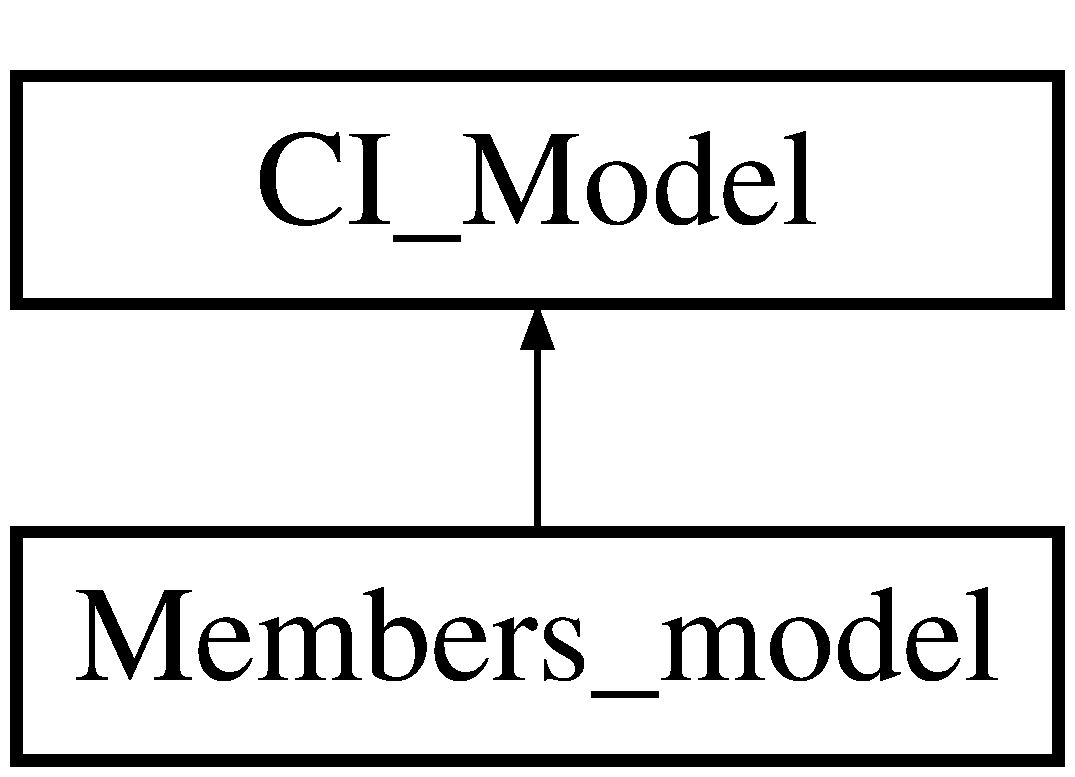
\includegraphics[height=2.000000cm]{classMembers__model}
\end{center}
\end{figure}
\subsection*{Public Member Functions}
\begin{DoxyCompactItemize}
\item 
\hyperlink{classMembers__model_a3d7a3e4e993f06c4926e256d8566501f}{get\-All} ()
\begin{DoxyCompactList}\small\item\em Busca no banco o cadastro completo de todos os membros. \end{DoxyCompactList}\item 
\hyperlink{classMembers__model_aa554c3ab3c6c4bb923f25b17239fe8cf}{insert\-Member} (\$name\-\_\-foto=null)
\item 
\hyperlink{classMembers__model_abf70725e69dada91ea0141868842f999}{get\-Areas} ()
\begin{DoxyCompactList}\small\item\em Busca as Areas disponiveis para casdrasto. \end{DoxyCompactList}\item 
\hyperlink{classMembers__model_a2e6bd5ec11b61b6bc6b96f6a9a6f711c}{get\-Privilegios} ()
\begin{DoxyCompactList}\small\item\em Busca os privilegios disponiveis para cadrastro. \end{DoxyCompactList}\item 
\hypertarget{classMembers__model_a3917f787e9a90de13f9bcea64c794798}{\hyperlink{classMembers__model_a3917f787e9a90de13f9bcea64c794798}{update\-Member} (\$edit\-Member)}\label{classMembers__model_a3917f787e9a90de13f9bcea64c794798}

\begin{DoxyCompactList}\small\item\em Faz o update dos cadastros no banco. \end{DoxyCompactList}\item 
\hyperlink{classMembers__model_a7d653a5e0a3ab26a042f37d213f94efb}{delete\-Member} (\$edit\-Member)
\end{DoxyCompactItemize}


\subsection{Detailed Description}
Busca, cadastra, edita, apaga e valida os usuarios no banco. 

\subsection{Member Function Documentation}
\hypertarget{classMembers__model_a7d653a5e0a3ab26a042f37d213f94efb}{\index{Members\-\_\-model@{Members\-\_\-model}!delete\-Member@{delete\-Member}}
\index{delete\-Member@{delete\-Member}!Members_model@{Members\-\_\-model}}
\subsubsection[{delete\-Member}]{\setlength{\rightskip}{0pt plus 5cm}Members\-\_\-model\-::delete\-Member (
\begin{DoxyParamCaption}
\item[{}]{\$edit\-Member}
\end{DoxyParamCaption}
)}}\label{classMembers__model_a7d653a5e0a3ab26a042f37d213f94efb}
Deleta os membros do banco. 
\begin{DoxyParams}{Parameters}
{\em edit\-Member} & \\
\hline
\end{DoxyParams}
\hypertarget{classMembers__model_a3d7a3e4e993f06c4926e256d8566501f}{\index{Members\-\_\-model@{Members\-\_\-model}!get\-All@{get\-All}}
\index{get\-All@{get\-All}!Members_model@{Members\-\_\-model}}
\subsubsection[{get\-All}]{\setlength{\rightskip}{0pt plus 5cm}Members\-\_\-model\-::get\-All (
\begin{DoxyParamCaption}
{}
\end{DoxyParamCaption}
)}}\label{classMembers__model_a3d7a3e4e993f06c4926e256d8566501f}


Busca no banco o cadastro completo de todos os membros. 

Cria o objeto Member

\begin{DoxyReturn}{Returns}
members\-List 
\end{DoxyReturn}
\hypertarget{classMembers__model_abf70725e69dada91ea0141868842f999}{\index{Members\-\_\-model@{Members\-\_\-model}!get\-Areas@{get\-Areas}}
\index{get\-Areas@{get\-Areas}!Members_model@{Members\-\_\-model}}
\subsubsection[{get\-Areas}]{\setlength{\rightskip}{0pt plus 5cm}Members\-\_\-model\-::get\-Areas (
\begin{DoxyParamCaption}
{}
\end{DoxyParamCaption}
)}}\label{classMembers__model_abf70725e69dada91ea0141868842f999}


Busca as Areas disponiveis para casdrasto. 

\begin{DoxyReturn}{Returns}
areas 
\end{DoxyReturn}
\hypertarget{classMembers__model_a2e6bd5ec11b61b6bc6b96f6a9a6f711c}{\index{Members\-\_\-model@{Members\-\_\-model}!get\-Privilegios@{get\-Privilegios}}
\index{get\-Privilegios@{get\-Privilegios}!Members_model@{Members\-\_\-model}}
\subsubsection[{get\-Privilegios}]{\setlength{\rightskip}{0pt plus 5cm}Members\-\_\-model\-::get\-Privilegios (
\begin{DoxyParamCaption}
{}
\end{DoxyParamCaption}
)}}\label{classMembers__model_a2e6bd5ec11b61b6bc6b96f6a9a6f711c}


Busca os privilegios disponiveis para cadrastro. 

\begin{DoxyReturn}{Returns}
Privilegios 
\end{DoxyReturn}
\hypertarget{classMembers__model_aa554c3ab3c6c4bb923f25b17239fe8cf}{\index{Members\-\_\-model@{Members\-\_\-model}!insert\-Member@{insert\-Member}}
\index{insert\-Member@{insert\-Member}!Members_model@{Members\-\_\-model}}
\subsubsection[{insert\-Member}]{\setlength{\rightskip}{0pt plus 5cm}Members\-\_\-model\-::insert\-Member (
\begin{DoxyParamCaption}
\item[{}]{\$name\-\_\-foto = {\ttfamily null}}
\end{DoxyParamCaption}
)}}\label{classMembers__model_aa554c3ab3c6c4bb923f25b17239fe8cf}
Insere os cadastro de um novo membro no banco. 
\begin{DoxyParams}{Parameters}
{\em name\-\_\-foto} & \\
\hline
\end{DoxyParams}
Inserio primeiro na tabela login.

Depois na tabela cadastro.

Depois na tabela fotos.

caso insira com sucesso em todas\-: \begin{DoxyReturn}{Returns}
True 
\end{DoxyReturn}


The documentation for this class was generated from the following file\-:\begin{DoxyCompactItemize}
\item 
application/models/\hyperlink{members__model_8php}{members\-\_\-model.\-php}\end{DoxyCompactItemize}

\hypertarget{classWelcome}{\section{Welcome Class Reference}
\label{classWelcome}\index{Welcome@{Welcome}}
}


Nativa do Codeigniter.  


Inheritance diagram for Welcome\-:\begin{figure}[H]
\begin{center}
\leavevmode
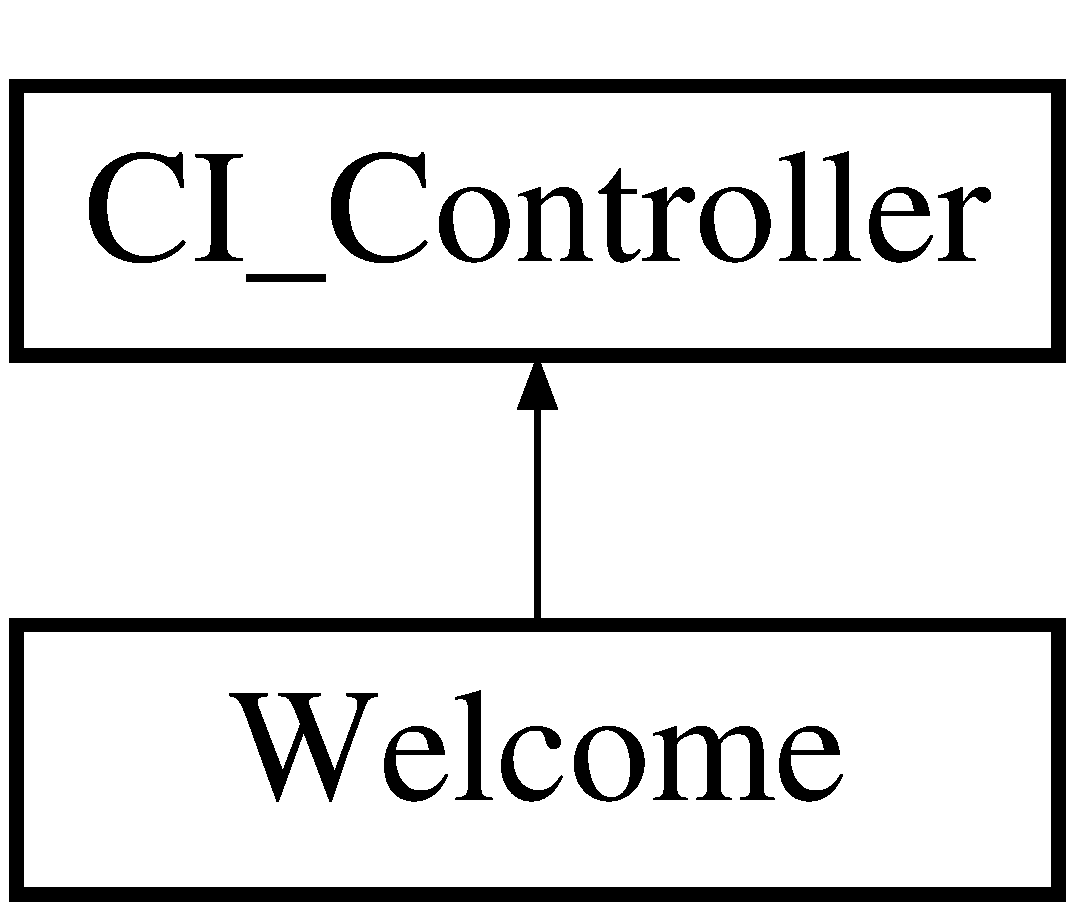
\includegraphics[height=2.000000cm]{classWelcome}
\end{center}
\end{figure}
\subsection*{Public Member Functions}
\begin{DoxyCompactItemize}
\item 
\hyperlink{classWelcome_a8aadbfbd06b65a6538badbed8569b293}{index} ()
\end{DoxyCompactItemize}


\subsection{Detailed Description}
Nativa do Codeigniter. 

\subsection{Member Function Documentation}
\hypertarget{classWelcome_a8aadbfbd06b65a6538badbed8569b293}{\index{Welcome@{Welcome}!index@{index}}
\index{index@{index}!Welcome@{Welcome}}
\subsubsection[{index}]{\setlength{\rightskip}{0pt plus 5cm}Welcome\-::index (
\begin{DoxyParamCaption}
{}
\end{DoxyParamCaption}
)}}\label{classWelcome_a8aadbfbd06b65a6538badbed8569b293}
Index Page for this controller.

Maps to the following U\-R\-L \href{http://example.com/index.php/welcome}{\tt http\-://example.\-com/index.\-php/welcome}
\begin{DoxyItemize}
\item or -\/ \href{http://example.com/index.php/welcome/index}{\tt http\-://example.\-com/index.\-php/welcome/index}
\item or -\/ Since this controller is set as the default controller in config/routes.\-php, it's displayed at \href{http://example.com/}{\tt http\-://example.\-com/}
\end{DoxyItemize}

So any other public methods not prefixed with an underscore will map to /index.php/welcome/$<$method\-\_\-name$>$ \begin{DoxySeeAlso}{See Also}
\href{http://codeigniter.com/user_guide/general/urls.html}{\tt http\-://codeigniter.\-com/user\-\_\-guide/general/urls.\-html} 
\end{DoxySeeAlso}


The documentation for this class was generated from the following file\-:\begin{DoxyCompactItemize}
\item 
application/controllers/welcome.\-php\end{DoxyCompactItemize}

\chapter{File Documentation}
\hypertarget{login_8php}{\section{application/controllers/login.php File Reference}
\label{login_8php}\index{application/controllers/login.\-php@{application/controllers/login.\-php}}
}


Sistema de login do canvas.  


\subsection*{Classes}
\begin{DoxyCompactItemize}
\item 
class \hyperlink{classLogin}{Login}
\begin{DoxyCompactList}\small\item\em Soliciata a realização do login e logout. \end{DoxyCompactList}\end{DoxyCompactItemize}


\subsection{Detailed Description}
Sistema de login do canvas. \begin{DoxyDate}{Date}
Set 30, 2014 
\end{DoxyDate}
\begin{DoxyAuthor}{Author}
thais Alencar 
\end{DoxyAuthor}

\hypertarget{members_8php}{\section{application/controllers/members.php File Reference}
\label{members_8php}\index{application/controllers/members.\-php@{application/controllers/members.\-php}}
}


Sistema de login do canvas.  


\subsection*{Classes}
\begin{DoxyCompactItemize}
\item 
class \hyperlink{classMembers}{Members}
\begin{DoxyCompactList}\small\item\em Mostra, cadastra, edita, apaga e valida os usuarios. \end{DoxyCompactList}\end{DoxyCompactItemize}


\subsection{Detailed Description}
Sistema de login do canvas. \begin{DoxyDate}{Date}
Set 30, 2014 
\end{DoxyDate}
\begin{DoxyAuthor}{Author}
thais Alencar 
\end{DoxyAuthor}

\hypertarget{login__model_8php}{\section{application/models/login\-\_\-model.php File Reference}
\label{login__model_8php}\index{application/models/login\-\_\-model.\-php@{application/models/login\-\_\-model.\-php}}
}


Sistema de login do canvas.  


\subsection*{Classes}
\begin{DoxyCompactItemize}
\item 
class \hyperlink{classLogin__model}{Login\-\_\-model}
\begin{DoxyCompactList}\small\item\em realização do login e logout. \end{DoxyCompactList}\end{DoxyCompactItemize}


\subsection{Detailed Description}
Sistema de login do canvas. \begin{DoxyDate}{Date}
Set 30, 2014 
\end{DoxyDate}
\begin{DoxyAuthor}{Author}
thais Alencar 
\end{DoxyAuthor}

\hypertarget{members__model_8php}{\section{application/models/members\-\_\-model.php File Reference}
\label{members__model_8php}\index{application/models/members\-\_\-model.\-php@{application/models/members\-\_\-model.\-php}}
}


Sistema de login do canvas.  


\subsection*{Classes}
\begin{DoxyCompactItemize}
\item 
class \hyperlink{classMembers__model}{Members\-\_\-model}
\begin{DoxyCompactList}\small\item\em Busca, cadastra, edita, apaga e valida os usuarios no banco. \end{DoxyCompactList}\end{DoxyCompactItemize}


\subsection{Detailed Description}
Sistema de login do canvas. \begin{DoxyDate}{Date}
Set 30, 2014 
\end{DoxyDate}
\begin{DoxyAuthor}{Author}
thais Alencar 
\end{DoxyAuthor}

%--- End generated contents ---

% Index
\newpage
\phantomsection
\addcontentsline{toc}{chapter}{Index}
\printindex

\end{document}
